\documentclass[lang=cn,10pt]{elegantbook}
\usepackage{subcaption}


\newcommand\bv[1]{\boldsymbol{#1}}
\newcommand\mb[1]{\mathbb{#1}}
\newcommand\mc[1]{\mathcal{#1}}

% \title{Complex Analysis}
% \subtitle{Elegant\LaTeX{} 经典之作}

\author{Lollins}
% \institute{Elegant\LaTeX{} Program}
\date{\today}
% \version{4.3}
% \bioinfo{自定义}{信息}

\extrainfo{改变人生的事情,你必须冒险;
	意义非凡的事情,大多碰巧发生;
	不重要的事,才有周全的计划。
}

\setcounter{tocdepth}{3}

\logo{logo1.jpg}
\cover{new.jpg}

% 本文档命令
\usepackage{array}
\newcommand{\ccr}[1]{\makecell{{\color{#1}\rule{1cm}{1cm}}}}

% 修改标题页的橙色带
% \definecolor{customcolor}{RGB}{32,178,170}
% \colorlet{coverlinecolor}{customcolor}

\begin{document}

\title{数学分析}
\author{Lollins}
\date{\today}

\maketitle

\pagenumbering{roman}
\setcounter{page}{1}

\begin{center}
    \Huge\textbf{前言}
\end{center}
\par
$2023/8/17$,发现用\LaTeX 做笔记还挺舒服的,以前喜欢用iPad,觉得手写的东西记得还牢固。但是iPad电池有问题,而且自己字写的好丑,不想用iPad了。\LaTeX 的格式真没话说,用起来很舒服。


这篇文章我来写一点关于数学分析中,可能被我遗忘掉了的知识点。

本笔记主要参考中科大程艺老师的《数学分析讲义》。


\begin{flushright}
    \begin{tabular}{c}
        Lollins \\
        \today
    \end{tabular}
\end{flushright}

\newpage
\pagenumbering{Roman}
\setcounter{page}{1}
\tableofcontents
\newpage
\setcounter{page}{1}
\pagenumbering{arabic}

\chapter{极限}

\chapter{单变量函数的连续性}

\chapter{单变量函数的微分学}

\chapter{不定积分}

\chapter{单变量函数的积分学}

\section{变上限积分}
\begin{theorem}
    对于函数$I(x)=\int_{0}^{g(x)}f(t)dt$,我们有$I'(x) = g'(x)f(x)$
\end{theorem}


\chapter{常微分方程初步}
\chapter{无穷级数}
\chapter{空间解析几何}
\chapter{多变量函数的微分学}
\section{方向导数与梯度}
\begin{definition}[叉乘]\label{de9.1}
    对于向量$\bv{a,b}$,定义叉乘为
    \begin{equation*}
        \begin{aligned}
            \bv{a}\times \bv{b} & =
            \begin{vmatrix}
                \vec{i} &  & \vec{j} &  & \vec{k} \\
                a_1     &  & a_2     &  & a_3     \\
                b_1     &  & b_2     &  & b_3
            \end{vmatrix} \\
                                & =
            \begin{vmatrix}
                a_2 & a_3 \\
                b_2 & b_3
            \end{vmatrix}
            \mathbf{i}+
            \begin{vmatrix}
                a_3 & a_1 \\
                b_3 & b_1
            \end{vmatrix}
            \mathbf{j}+
            \begin{vmatrix}
                a_1 & a_2 \\
                b_1 & b_2
            \end{vmatrix}
            \mathbf{k}
        \end{aligned}
    \end{equation*}
\end{definition}

\begin{definition}[方向导数]
    对于$\bv{e} = \bv{i}~cos\alpha+\bv{j}~sin\alpha,f(x,y)$,如果极限
    \begin{equation}
        \begin{aligned}
            \lim_{t\to0}\frac{f(x+t\cos\alpha,y+t\sin\alpha)-f(x,y)}t
        \end{aligned}
    \end{equation}
    存在,那么称极限值为$f$在点$(x,y)$沿方向$\bv{e}$的方向导数,记为$\frac{\partial f}{\partial \bv{e}}(x,y)$。
\end{definition}

\begin{theorem}
    设$f(x,y)$是平面区域$D$上的可微函数,则$f(x,y)$在$D$上任何一点沿方向
    $\bv{e} = \bv{i}~cos\alpha+j~sin\alpha$的方向导数都存在,而且有
    \begin{equation}
        \begin{aligned}
            \frac{\partial f}{\partial e}=\frac{\partial f}{\partial x}\cos\alpha+\frac{\partial f}{\partial y}sin\alpha
        \end{aligned}
    \end{equation}
\end{theorem}

\begin{definition}[梯度]
    对于$\bv{e} = \bv{i}~cos\alpha+\bv{j}~sin\alpha,f(x,y)$,记
    \begin{equation}
        \mathrm{grad}f=\frac{\partial f}{\partial x}\bv{i}+\frac{\partial f}{\partial y}\bv{j}
    \end{equation}
    为$f$在点$(x,y)$处的梯度。
\end{definition}

因此函数沿任何方向的方向导数为该方向与函数的梯度的内积($\theta$为$\mathrm{grad}f\text{和} e$之间的夹角)
,即
\begin{equation}
    \frac{\partial f}{\partial e} = \mathrm{grad}f\cdot e=|\mathrm{grad}f| |e|cos\theta
\end{equation}

\chapter{多变量函数的重积分}

\chapter{曲线积分和曲面积分}
\section{数量场在曲线上的积分}
\begin{theorem}
    设$L$是空间上的一条光滑曲线,其参数方程表示为
    \begin{equation}
        \bv{r}=\bv{r}(t)=x(t)\boldsymbol{i}+y(t)\boldsymbol{j}+z(t)\boldsymbol{k}\quad t\in[\alpha,\beta]
    \end{equation}
    $\phi(x,y,z)$在$L$上连续,则$\phi(x,y,z)$在曲线$L$上可积,且
    \begin{equation*}
        \begin{aligned}
            \int_{L}\phi(x,y,z)\mathrm{d}s
             & =\int_\alpha^\beta\phi(x(t),y(t),z(t))|\boldsymbol{r}^\prime(t)|\mathrm{d}t                                    \\
             & =\int_\alpha^\beta\phi(x(t),y(t),z(t))\sqrt{x^{\prime{'}^2}(t)+{y^{\prime}}^2(t)+{z^{\prime}}^2(t)}\mathrm{d}t
        \end{aligned}
    \end{equation*}
\end{theorem}

\begin{example}
    求曲线积分$\int_Lxyds$。其中$L$为椭圆$\frac{x^2}{a^2}+\frac{y^2}{b^2}=1$
    在第一象限上的弧段。
\end{example}
\begin{solution}
    $L$的方程可写为
    \begin{equation*}
        x=a\cos\theta,\quad y=b\sin\theta,\quad0\leqslant\theta\leqslant\frac\pi2,
    \end{equation*}
    所以
    \begin{equation*}
        \begin{aligned}
            \int_{L}xy\mathrm{d}s &
            \begin{aligned}
                 & =ab\int_0^{\pi/2}\cos\theta\sin\theta\sqrt{a^2\sin^2\theta+b^2\cos^2\theta}\mathrm{d}\theta
            \end{aligned}                    \\
                                  & =\frac{ab}2\int_0^{\pi/2}\sqrt{b^2+(a^2-b^2)\sin^2\theta}\text{ d}\sin^2\theta            \\
                                  & =\frac{ab}{3(a^2-b^2)}\left.\left(b^2+(a^2-b^2)\sin^2\theta\right)^{3/2}\right|_0^{\pi/2} \\
                                  & =\frac{ab(a^2+ab+b^2)}{3(a+b)}
        \end{aligned}
    \end{equation*}
\end{solution}

\section{数量场在曲面上的积分}
\begin{theorem}
    设$S$是一张有界的光滑曲面,$\varphi(x,y,z)$是定义在$S$上的数量场,且在$S$上连续。设曲面的参数方程为
    \begin{equation}
        \bv{r}=\bv{r}(u,v)=x(u,v)\boldsymbol{i}+y(u,v)\boldsymbol{j}+z(u,v)\boldsymbol{k},\quad(u,v)\in D,
    \end{equation}
    则$\varphi(x,y,z)$在$S$上可积,为
    \begin{equation*}
        \begin{aligned}
            \iint_{S}\varphi(x,y,z)\mathrm{d}S
             & =\iint_D\varphi(x(u,v),y(u,v),z(u,v))|\boldsymbol{r}_u^{\prime}\times\boldsymbol{r}_v^{\prime}|\mathrm{d}u\mathrm{d}v \\
             & =\iint_{D}\varphi(x(u,v),y(u,v),z(u,v))\sqrt{EG-F^{2}}\mathrm{d}u\mathrm{d}v
        \end{aligned}
    \end{equation*}
    其中$\boldsymbol{r}_u^{\prime}\times\boldsymbol{r}_v^{\prime}$为向量叉乘(参考定义\ref{de9.1}),以及
    \begin{equation*}
        \begin{aligned}
            E & ={r'}_u^2={x'}_u+{y'}_u+{z'}_u,                \\
            G & ={r'}_v^2={x'}_v^2+{y'}_v+{z'}_v,              \\
            F & ={r'}_u\cdot {r'}_v=x'_ux'_v+y'_uy'_v+z'_uz'_v
        \end{aligned}
    \end{equation*}
\end{theorem}

\begin{example}
    设$S$是第一卦限的球面,$x^2+y^2+z^2=R^2\left(x\geqslant0,y\geqslant0,z\geqslant0\right)$,
    计算曲面积分$\iint_S(x^2+y^2)dS$。
\end{example}

\begin{solution}
    将球面$S$表示为参数方程
    \begin{equation*}
        x=R\sin\theta\cos\varphi,y=R\sin\theta\sin\varphi,z=R\cos\theta,
    \end{equation*}
    则$\theta,\varphi$的变化范围是平面$O'\theta\varphi$上的矩形$D'$
    \begin{equation*}
        0\leqslant\theta\leqslant\frac{\pi}{2},\quad0\leqslant\varphi\leqslant\frac{\pi}{2},
    \end{equation*}
    所以
    \begin{equation*}
        \begin{aligned}
            \iint_{S}(x^{2}+y^{2})\mathrm{d}S
             & =\iint_{D^{\prime}}R^2\sin^2\theta\cdot R^2\sin\theta\mathrm{d}\theta\mathrm{d}\varphi \\
             & =R^4\int_0^{\frac\pi2}\mathrm{d}\varphi\int_0^{\frac\pi2}\sin^3\theta\mathrm{d}\theta  \\
             & =\frac{1}{3}\pi R^4
        \end{aligned}
    \end{equation*}
\end{solution}

\section{向量场在曲线上的积分}
\begin{theorem}
    设向量场$\bv{v}=P(x,y,z)\boldsymbol{i}+Q(x,y,z)\boldsymbol{j}+R(x,y,z)\boldsymbol{k}$在区域$D$上连续,
    曲线$L_{AB} \subset D$具有参数方程表示
    \begin{equation}
        L_{AB}:\quad\boldsymbol{r}=\boldsymbol{r}(t)=x(t)\boldsymbol{i}+y(t)\boldsymbol{j}+z(t)\boldsymbol{k},
        \quad\alpha\leqslant t\leqslant\beta,
    \end{equation}
    且有连续的导函数,参数t是正向参数,则向量场在$L_{AB}$上可积,且可化为下列定积分
    \begin{equation}
        \begin{aligned}
            \int_{L_{AB}}v\cdot\mathrm{d}r
             & =\int_{\alpha}^{\beta}v(r(t))\cdot r^{\prime}(t)\mathrm{d}t \\
             & =\int_{\alpha}^{\beta}(Px'(t)+Qy'(t)+Rz'(t))\mathrm{d}t
        \end{aligned}
    \end{equation}
\end{theorem}

\begin{example}
    计算曲线积分$\int_{L}xy\mathrm{d}x+x^{2}\mathrm{d}y,L$是三角形$OAB$的正向周界(如图\ref{im11_1}),
    其中$A(1,0),B(1,2),O(0,0)$。
    \begin{figure}[ht]
        \centering
        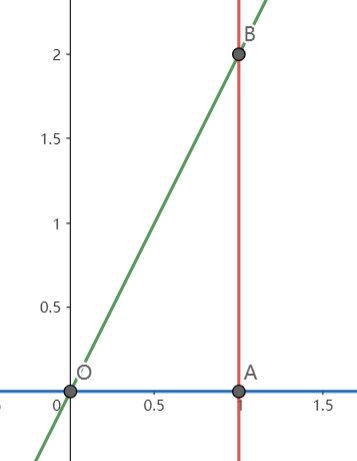
\includegraphics[width = 6cm]{img/im11_1.png}
        \caption{}
        \label{im11_1}
    \end{figure}
\end{example}

\begin{solution}
    因为
    \begin{equation*}
        \begin{gathered}
            \int_{L}xy\mathrm{d}x+x^2\mathrm{d}y =\int_{L_{1}}xy\mathrm{d}x+x^{2}\mathrm{d}y+\int_{L_{2}}xy\mathrm{d}x+x^{2}\mathrm{d}y \\
            +\int_{L_3}xy\mathrm{d}x+x^2\mathrm{d}y,
        \end{gathered}
    \end{equation*}
    在$L_1$上,$y=0,dy=0,x$是参变量,$0\leq x \leq 1$,所以
    \begin{equation*}
        \int_{L_1}xy\mathrm{d}x+x^2\mathrm{d}y=\int_0^1x\cdot0\mathrm{d}x=0;
    \end{equation*}
    在$L_2$上,$x=1,dx=0,y$是参变量,$0\leq y \leq 2$,所以
    \begin{equation*}
        \int_{L_2}xy\mathrm{d}x+x^2\mathrm{d}y=\int_0^21\cdot\mathrm{d}y=2;
    \end{equation*}
    在$L_3$上,$y=2x,0\leq x \leq 1,x$是参变量,所以
    \begin{equation*}
        \begin{aligned}
            \int_{L_3}xy\mathrm{d}x+x^2\mathrm{d}y & =\int_1^0x\cdot2x\mathrm{d}x+x^2\mathrm{d}(2x)=-\frac43
        \end{aligned}
    \end{equation*}
    从而算得
    \begin{equation*}
        \int_Lxy\operatorname{d}x+x^2\operatorname{d}y=\frac23
    \end{equation*}
\end{solution}



\section{向量场在曲面上的积分}



\chapter{Fourier分析}
\chapter{反常积分和含参变量积分}
\chapter{实属理论}

\chapter{连续性与收敛性}
\chapter{度量空间的连续函数}
\chapter{映射的微分}
\chapter{Riemann积分}



\end{document}
